\documentclass[11pt]{article}
\usepackage[utf8]{inputenc}
\usepackage[T1]{fontenc}
\usepackage{grffile}
\usepackage{longtable}
\usepackage{wrapfig}
\usepackage{rotating}
\usepackage[normalem]{ulem}
\usepackage{amsmath}
\usepackage{textcomp}
\usepackage{amssymb}
\usepackage{capt-of}
\usepackage{hyperref}
\hypersetup{colorlinks=true, linkcolor=magenta, citecolor=cyan}
\setlength{\parindent}{0in}
\usepackage[margin=1in]{geometry}
\usepackage[english]{babel}
\usepackage{mathtools}
\usepackage{palatino}
\usepackage{fancyhdr}
\usepackage{sectsty}
\usepackage{engord}
\usepackage{parskip}
\usepackage{minted}
\usepackage{graphicx}
\usepackage{subcaption}
\usepackage{setspace}
%\usepackage[center]{caption}
\usepackage{placeins}
\usepackage{color}
\usepackage{amsmath}
\usepackage{bm}
\usepackage{todonotes}
\usepackage{pdfpages}
% \titlespacing*{\subsection}{0pt}{5.5ex}{3.3ex}
%\titlespacing*{\section}{0pt}{5.5ex}{1ex}
\usepackage{natbib}
\setcitestyle{authoryear,aysep={,}}

\author{Luis Antonio Ortega Andrés\\Antonio Coín Castro}
\date{\today}
\title{DeepFakes Detection Lab - Report}
\hypersetup{
 pdfauthor={Luis Antonio Ortega Andrés, Antonio Coín Castro},
 pdftitle={},
 pdfkeywords={},
 pdfsubject={},
 pdflang={English}
 }

\begin{document}

\maketitle

\section*{Task 1: intra-database analysis}

\textit{The goal of this task is to develop and evaluate DeepFake detection systems over the same database. In this task, you should use only the UADFV database, which is divided into \texttt{development} and \texttt{evaluation} datasets.}

The notebook associated with this task is \texttt{Task1-2.ipynb}.

\textbf{a)} \textit{Provide all details (including links or references if needed) of your proposed DeepFake detection system.}

Our DeepFake detection system consists on the following modules:
\subsection*{Preprocessing}

First of all, the given images from UADFV have been preprocessed following these steps:
\begin{enumerate}
  \item The data is loaded using \texttt{Keras}' \texttt{flow\_from\_directory} function \citep{chollet2015keras}, so that we don't have to keep all images in memory while training our model. We resize each image to a resolution of $768\times 768$.
  \item We use the MTCNN face detector \citep{zhang2016joint} in order to crop the section of the image that contains the face. The aim of this phase is to erase those parts of the image that are not relevant for our classification task.
  \item We add random noise to the images as a form of regularization, to force our classifier to learn more relevant features. More precisely, we randomly decide wether the image is slightly blurred using a Gaussian filter from OpenCV \citep{opencv_library}, or simply perturbed by Gaussian noise. Each of these outcomes is equally likely and every image goes through one or the other, but never both. Note that these perturbations are only applied to training samples and not to the evaluation images.
\end{enumerate}

\subsection*{Feature extraction}

We decided that the best way of extracting features from the faces was \texttt{dlib}'s 68-point face landmark detector \citep{dlib09}. For each (cropped) face image, we obtain the spatial position of the 68 landmarks, and our final feature vector is composed of the gray-scale intensities of these landmarks. We then center each feature vector to have zero mean.

We also considered the possibility of applying PCA for dimensionality reduction, but since we wanted to try both approaches, we delegated this decision to the actual training step.

\subsection*{Classifier}

The final step of our model is a machine learning model that acts as a classifier to which the feature vectors are fed for training. At first we considered four distinct families of models for this job: \textbf{Linear SVM}, \textbf{SVM with RBF kernel}, \textbf{2-layer perceptron} and \textbf{Logistic Regression} models. The process by which a final classifier was selected can be seen on the next section.

\textbf{b)} \textit{Provide all details of the development/training procedure followed and the results achieved using the development dataset of the UADFV database. Show the results achieved in terms of Receiver Operating Characteristic (ROC) curve and Area Under the Curve (AUC).}

For the training procedure we performed a hyperparameter grid search using \texttt{Sklearn}'s API \citep{sklearn_api}, in which each family of classifiers mentioned above is tested with a wide range of possible hyperparameters to maximize the AUC metric. For example, the number and size of the hidden layers considered for the MLP are \( \{(50), (100), (50, 50), (100, 100)\} \), and the linear SVM regularization term \( C \) varies from \( 10^{-3} \) to \( 10^{3} \) with 40 equidistant steps. To make the process fair, we employ \textbf{5-fold cross validation} to select the best hyperparameters for each model, and in the end we select the model that achieved the highest cross-validated AUC. Note that each family of classifiers is trained using the same folds, so the results are comparable.

Before completing the training pipeline, we added the possibility to train each classifier \textbf{with and without PCA reduction}, to see whether it would have a positive impact on the final result. The fraction of explained variance to be retained was also an hyperparameter, whose search space was $\{0.90, 0.95, 0.99\}$. An important detail is that the data is first standardized to have zero mean and unit variance, since we observed that the performance of the classifiers was noticeably better after this normalization.

The best models of each family after running the grid search are shown in Table \ref{tab:t1}, along with their cross-validated AUC scores.

\begin{table}[H]
  \centering
  \begin{tabular}{llll}
    \textbf{Model}      & \textbf{PCA} & \textbf{Parameters} & \textbf{AUC (CV)} \\ \hline
    SVM RBF             & No &      \( C = 1.6681, \, \gamma = 0.0167\)  &     \( {\color{blue!80!black}{0.9937}} \)       \\
    SVM Linear          & No &   \(  C = 0.0174 \)   &   \( 0.9186 \)   \\
    MLP                 & No  &  \(\alpha=0.2154, \,size=(100, 100) \)     &    \(  0.9883 \)          \\
    LR & No & \( C = 0.1624 \) &    \( 0.9180 \)
    \end{tabular}
    \caption{Results of the hyperparameter tuning phase.}
    \label{tab:t1}
  \end{table}

As we can see, the best performing model was the \textbf{non-linear SVM with RBF kernel using the raw features}, and this is the model that we choose as our final classifier (with the optimized parameters found). An interesting thing to note is that PCA was discarded on every model, probably because the number of raw features considered is not very high and the model wouldn't benefit from having less features. The results of evaluating our chosen model on the whole development set can be seen on Figure \ref{fig:t1-roc-train}, in which we see that we achieve a perfect score.

\begin{figure}[h!]
  \centering
  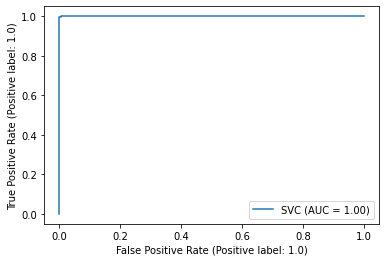
\includegraphics[width=.6\textwidth]{img/1-roc-UADFV-train}
  \caption{ROC curve and AUC value on UADFV's development set.}
  \label{fig:t1-roc-train}
\end{figure}

\textbf{c)} \textit{Describe the final evaluation of your proposed DeepFake detection system and the results achieved using the evaluation dataset (not used for training). Show the results achieved in terms of ROC curve and AUC. Provide an explanation of your results.}

Having chosen our model, we simply evaluate it on the previously unseen evaluation set of the UADFV database, and the results can be seen in Figure \ref{fig:t1-roc-test}. We obtain an AUC of $0.95$, quite close to the perfect score of $1.0$. Since there was no sudden drop in the performance of the model, it is safe to assume that the distribution of the evaluation set is more or less the same as that of the development set (as it should be). We can say that we have succeeded in this task, since our model has learned to detect DeepFakes on the UADFV database while avoiding overfitting.

\begin{figure}[h!]
  \centering
  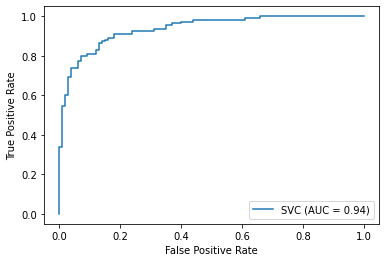
\includegraphics[width=.6\textwidth]{img/1-roc-UADFV}
  \caption{ROC curve and AUC value on UADFV's evaluation set.}
  \label{fig:t1-roc-test}
\end{figure}

\subsection*{Other approaches and failed attempts}

\begin{enumerate}
  \item We considered extracting features using an image destriptor such as SURF or SIFT, and then following the Bag of Visual Words technique. However, the results obtained were worse, so we discarded this approach.
  \item Along with the landmarks intensity, we made some attempts at using the the landmarks locations as features, but this resulted in overfitting. As a regularization technique, we tried to center those locations (substracting the mean) in order to make them location invariant. The performance improved a bit but the overall model was still worse, so in the end we decided to stick to the landmarks intensity only.
  \item At one point, MTCNN did not correctly detect the faces for every image, and during training we decided to simply skip these images. However, since we cannot skip test cases, we decided that an image with no face detected would be assumed to have the same features as the last image with the same label. In the end we solved the underlying problem (by resizing the input images), but we left all the code checks just in case they were needed in the future.
  \item More models were tested in the grid search, such as Random Forests and other boosting techniques. However, they performed so poorly compared to the rest that we decided not to include them in the final report.
\end{enumerate}

\section*{Task 2: inter-database analysis}

\textit{The goal of this task is to evaluate the DeepFake detection system developed in Task 1 with a new database (not seen during the development/training of the detector). In this task, you should use only the Celeb-DF. You only need to evaluate your fake detector developed in Task 1 over the \texttt{evaluation} dataset of Celeb-DF, not train again with them.}

The notebook associated with this task is \texttt{Task1-2.ipynb}.

\textbf{a)} \textit{Describe the results achieved by your DeepFake detection system developed in Task 1 using the evaluation dataset of the Celeb-DF database. Show the results achieved in terms of ROC curve and AUC. Provide an explanation of your results in comparison with the results of Task 1.}

We evaluate the model established in the previous task (SVM with RBF kernel and optimized hyperparameters) on the evaluation set of Celeb-DF. The results achieved can be seen in Figure \ref{fig:t2}.

\begin{figure}[h!]
  \centering
  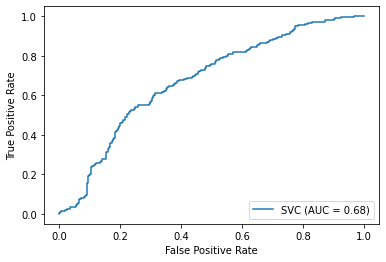
\includegraphics[width=.6\textwidth]{img/2-roc-celeb}
  \caption{ROC curve and AUC value on Celeb-DF's evaluation set.}
  \label{fig:t2}
\end{figure}

We obtain an AUC of 0.64, which is considerably lower than the one achieved in the previous task. This behaviour makes sense, considering that the training dataset was less challenging than this one, in the sense that the deepfakes were more easily spotted by a human. In the UADFV dataset there were usually vertical and horizontal strips surrounding the place where the face exchange had taken place, and in this new dataset deepfakes have a higher quality and do not show such markings. In short, our detection model scales poorly to this dataset because the data in which it was trained \textbf{is not representative enough} of this new evaluation set.


\section*{Task 3: inter-database proposal}

\textit{The goal of this task is to improve the DeepFake detection system originally developed in Task 1 in order to achieve better inter-database results. You must consider the same evaluation dataset as in Task 2 (i.e. the \texttt{evaluation} dataset of the Celeb-DF database).}

\textbf{a)} \textit{Describe the improvements carried out in your proposed DeepFake detection system in comparison with Task 1.}

In the first place, we tried to increase the quantity of data we had to train our model. To build a new training set, we used the full given UADFV dataset (merging development and evaluation) and several samples of the DeepFakeTIMIT and VidTIMIT databases \citep{sanderson2009multi}. As DeepFakeTIMIT is composed of videos, we developed a python script in order to take frames from the videos (\texttt{TIMIT\_data\_preprocess.py}). Moreover, since these datasets have a relatively low diversity (only 32 different people appear on the videos), we decided not to take all the samples we could, but instead get a random sample of both real and fakes images while we cropped a \( 160 \times 160 \) face image using MTCNN (\texttt{Face\_detector\_splitter.py}).

After increasing the number of training samples, we followed different approaches in order to find and optimize the most suitable technique for this problem. In all cases the \textbf{training dataset} was composed of \( 1829 \) \( 160\times 160 \) face samples, and the \textbf{evaluation dataset} was composed of the \( 160 \times 160 \) face crops of each sample (out of 600) in the given \texttt{Celeb-DF} dataset. Although the MTCNN face detector remains an essential part of our model architecture, we saved the cropped faces to disk and worked only with them to increase the computational efficiency.

\subsection*{Train the same model with more data}

First of all, we wanted to check how the best model found in the previous task behaved with this new training dataset, and set a \emph{baseline} to be compared to the subsequent attempts.

The procedure was simple and can be seen in the notebook \texttt{Task3\_ML.ipynb}. We reused the majority of the code developed for the previous task and created a pipeline with the optimal classifier. The AUC obtained using this approach was 0.67, which is only a bit better that what we had before.

\subsection*{Consider alternative features}

In this approach we intended to use \texttt{FaceNet} \citep{Schroff_2015} to obtain a more representative set of features for each face. To this end, we took a pre-trained model of FaceNet\footnote{\url{https://github.com/nyoki-mtl/keras-facenet}} that computed a face embedding to \( 128 \) features, and used these features \textbf{along with the landmarks intensities} to train and cross-validate the same families of models considered in Task 1. A small change that we make is that we stop randomly blurring the training images, since we observed that it could heavily distort the embedding and worsen the performance of the final model.

The resulting best model was again the SVM with RBF kernel, using a regularization term \( C = 4.6415 \) and a kernel parameter \( \gamma = 0.0167 \). The AUC score on the evaluation dataset was \( 0.7 \), which is better than our baseline model.

The code for this strategy can be consulted in \texttt{Task3\_Facenet.ipynb}.

\subsection*{Train a deep learning model from scratch}

In this attempt we wanted to take advantage of the increased number of samples in the training dataset to use a \emph{deep-but-not-so-deep} convolutional neural network for the classification task. We considered a simple model consisting on  two blocks of convolution-activation-dropout-pooling and two fully connected layers at the end, the last one being a sigmoid with only one unit. We also used data augmentation techniques such as random rotations or horizontal flipping as an extra regularization layer.

However, after tuning the parameters for a while using a validation set and the early stopping technique, the model either overfitted to the training dataset or did not learn at all, so we discarded this approach altogether. The general structure with our experiments can be found in \texttt{Task3\_DL.ipynb}.

\subsection*{Fine-tune a pre-trained deep learning model}

As our last attempt, we aimed to fine-tune a pre-trained deep neural network. We thought that we could benefit from a large network that was already trained on a big database, and perform transfer learning to try to solve our detection problem. We used the \texttt{Keras} API and followed these steps\footnote{We followed the recommendations in \url{https://keras.io/guides/transfer_learning/}}:

\begin{enumerate}
  \item We loaded a CNN pre-trained on the ImageNet database \citep{deng2009imagenet}.  We tested several well-known models such as VGG19, ResNet50, InceptionV3, XceptionNet...
  \item We dropped the top layers that act as a classifier, and put a small fully connected model of our choosing instead.
  \item We train \textbf{only the top layers} on our dataset for a few epochs, so that the weights are correctly initialized and are not random. This is done to avoid disturbing the previously tuned weights of the base model.
  \item \textbf{We unfreeze the last convolutional block of the base model} and train with a small learning rate to perform the actual fine-tuning of the network. We don't unfreeze the whole network because the initial layers act as a coarse feature extractor, and our hypothesis was that the images on ImageNet share the same lower level features as our images. It is only on the last layers of the network that features close to our deepfake detection problem are learned, and that is where we put our efforts. Moreover, if we trained the whole network we would almost certainly incur in overfitting, since we have a very limited quantity of training data.
\end{enumerate}

We retain the random data augmentation technique from previous attempts, but we do not consider a validation set in this case, to try and make the most out of our few training examples. After some tries, the best configuration found was as follows:

\begin{itemize}
  \item The chosen base model was the VGG19 network \citep{simonyan2015deep}. We needed to add a preliminary preprocessing step to accomodate the images to VGG19's expectations (using the function \texttt{vgg19.preprocess\_input}).
  \item The top model chosen was a small model consisting on two fully connected layers with ReLu activation and 512 and 256 units respectively, with a Dropout layer of $0.25$ after the first one and another of $0.5$ after the second one. The Dropout layers are regularizing layers that ``turn off'' a fraction of the neurons during training, to force the model to learn more relevant features. At the end we put a Dense layer with one unit and sigmoid activation to obtain the probabilities of fake and real.
  \item We trained the top model for 3 epochs, and then unfroze the last convolutional block of VGG19 and trained for 15 more epochs, in this case using the SGD optimizer with a learning rate of $5\cdot 10^{-4}$.
\end{itemize}

The code developed can be consulted in the notebook \texttt{Task3\_Finetune.ipynb}.

\textbf{b)} \textit{Describe the results achieved by your enhanced DeepFake detection system over the final evaluation dataset. Show the results achieved in terms of ROC curve and AUC. Provide an explanation of your results in comparison with the results of Task 2.}

After evaluating the trained model on the evaluation dataset, we obtained a shocking AUC score of $0.8107$ , whose corresponding ROC curve can be seen in Figure \ref{fig:t3}. It turns out that this fine-tuning approach was the best way of enhancing our model, and we improved the results of Task 2 by almost 20 percentage points.

\begin{figure}[h!]
  \centering
  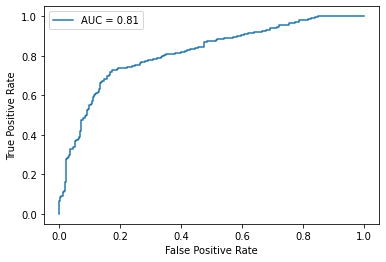
\includegraphics[width=.6\textwidth]{img/3-finetune-roc-celeb}
  \caption{ROC curve and AUC value on Celeb-DF's evaluation set for our enhanced model.}
  \label{fig:t3}
\end{figure}

\textbf{c)} \textit{Indicate the conclusions and possible future improvements}.

The conclusions we draw from this assignment are summarized below:

\begin{itemize}
  \item DeepFake detection is a challenging task, especially when there are more and more high-quality fakes that even humans have a hard time detecting. The fact that we train on a specific database and obtain good results is not a guarantee that the model will generalize to different databases.
  \item Feature extraction is a key part of the process, and the more relevant and accurate features we obtain, the better the performance of our final model.
  \item While we can obtain a decent performance using machine learning techniques, deep learning outperforms classical approaches when used appropriately.
  \item Deep learning is an excellent way to perform a sort of automatic feature extraction, letting the network learn which features are relevant for the specific task of deepfake detection. However, for this approach to succeed we generally need a large amount of training data.
  \item We can overcome the need for many training images using transfer learning and fine-tuning a pre-trained network, but we have to pay close attention to the process and employ a suite of regularization techniques to avoid overfitting.
\end{itemize}

As a final comment, we considered some alternative feature extraction techniques, but we didn't have time to implement them. For example, we thought it would be a good idea to obtain specific masks for different parts of the face, such as eyes, teeth, nose, etc, and in general to adopt a more fine-grained approach when it comes to feature extraction. Moreover, we thought it would be good to have an in-depth look at how deepfakes are usually generated (using GANs), and then try to exploit any weaknesses in the process to improve our detection performance.

We also tried to obtain more training samples from various databases such as FaceForensics++ \citep{rossler2018faceforensics}, but they were either hard to obtain or difficult to preprocess to suit our specific needs. Nonetheless, we think that having a bigger and more diverse training set would substantially increase the performance of the detection model.

%%%%%%%%%%%%%%%%
%% Bibliography
%%%%%%%%%%%%%%%%

\bibliographystyle{authordate1}
\bibliography{bibliography}

\end{document}
